\let\negmedspace\undefined
\let\negthickspace\undefined
\documentclass[journal,12pt,twocolumn]{IEEEtran}
\usepackage{cite}
\usepackage{amsmath,amssymb,amsfonts,amsthm}
\usepackage{algorithmic}
\usepackage{graphicx}
\usepackage{textcomp}
\usepackage{xcolor}
\usepackage{txfonts}
\usepackage{listings}
\usepackage{enumitem}
\usepackage{mathtools}
\usepackage{gensymb}
\usepackage{comment}
\usepackage[breaklinks=true]{hyperref}
\usepackage{tkz-euclide} 
\usepackage{listings}
\usepackage{gvv}                                        
\def\inputGnumericTable{}                                 
\usepackage[latin1]{inputenc}                                
\usepackage{color}                                            
\usepackage{array}                                            
\usepackage{longtable}                                       
\usepackage{calc}                                             
\usepackage{multirow}                                         
\usepackage{hhline}                                           
\usepackage{ifthen}                                           
\usepackage{lscape}

\newtheorem{theorem}{Theorem}[section]
\newtheorem{problem}{Problem}
\newtheorem{proposition}{Proposition}[section]
\newtheorem{lemma}{Lemma}[section]
\newtheorem{corollary}[theorem]{Corollary}
\newtheorem{example}{Example}[section]
\newtheorem{definition}[problem]{Definition}
\newcommand{\BEQA}{\begin{eqnarray}}
\newcommand{\EEQA}{\end{eqnarray}}
\newcommand{\define}{\stackrel{\triangle}{=}}
\theoremstyle{remark}
\newtheorem{rem}{Remark}
\begin{document}

\bibliographystyle{IEEEtran}
\vspace{3cm}

\title{11.9.3.3}
\author{EE23BTECH11065 - prem sagar}
\maketitle
\newpage

\bigskip
hi
\renewcommand{\thefigure}{\theenumi}
\renewcommand{\thetable}{\theenumi}
\textbf{Question}:\\ The 5th,8th and 11th terms of a GP are p,q and s respectively .show that \[q^2=ps\]
\textbf{solution}:
\\Given,
\begin{align}
x(5)=p
\\x(8)=q
\\x({11})=s
\end{align}
\\let first term of a GP= a\\
common ratio of GP=r
\\we know,
\begin{align}
\text{nth term of  a GP}=x(n)&= a\cdot r^{n}, \text{if} n \geq 0
\\\text{so 5th  term of GP}(x(5))&=a\cdot r^5=p
\\\text{8th  term  of  GP}(x(8))&=a\cdot r^8=q
\\\text{11th  term  of  GP}(x({11}))&=a\cdot r^{11}=s
\\x(8)\cdot x(8)=a\cdot r^8\cdot a\cdot r^8
     \\ =a^2\cdot r^{16}
\\x(5)\cdot x({11})=a\cdot r^5\cdot a\cdot r^{11}
       \\=a^2\cdot r^{16}
\\x(8)^2=x(5)\cdot x({11})
\end{align}
\\so,
\begin{align}
p=a\cdot r^5
\\q=a\cdot r^8
\\s=a\cdot r^{11}
\\q^2=p\cdot s
\end{align}
\\hence proved
\\\\\begin{tabular}{|c|c|c|}
\hline
\textbf{symbol}& \textbf{value}& \textbf{description}
\\\hline
\multirow{10}{1em}
\\$x(5)$ &$a\cdot r^5=p$& 5th term of GP 
\\$x(8)$ &$a\cdot r^8=q$& 8th term of GP 
\\$x({11})$ &$a\cdot r^{11}=s$& 11th term of GP
\\\hline
\end{tabular}\\
\\\\$u(n)=\begin{cases} 1,& \text{if} n\geq 0 \\\ 0,& \text{otherwise} \end{cases}$
\\\\\\\begin{align}x(n)=a\cdot r^{n}\cdot u(n)\end{align}
from (17)
\\\\$x(n)=\begin{cases} a\cdot r^{n} &\text{if} n \geq 0\\\ 0,& \text{otherwise}
\end{cases}$
\begin{figure}
    \centering
    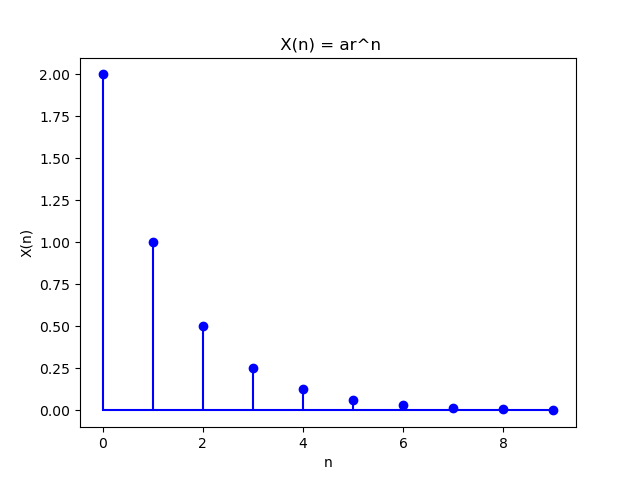
\includegraphics[width=1\linewidth]{/root/assign1/figs/geometric_sequence_plot.png}
    \caption{plot of x(n) vs n}
    \label{fig:enter-label}
\end{figure}
\\\\\begin{align}x(n)\overset{Z}{\longleftrightarrow}   X(Z)
\\X(Z)=\sum_{n=-\infty}^{\infty}x(n)\cdot Z^{-n}\
\end{align}
\\using (19)
\begin{align}
      =\sum_{n=-\infty}^{\infty}a\cdot r^{n}\cdot u(n)\cdot z^{-n}
     \\=a \sum_{n=-\infty}^{\infty} r^{n}\cdot u(n)\cdot z^{-n}\
       \\=a\sum_{n=0}^{\infty}r^{n}\cdot z^{-n}\
      \\ \text{sum of infinite terms in G.P}=\frac{a}{1-r}
     \end{align}
     from (23)
     \begin{align}
         =a\cdot \frac{1}{1-r\cdot z^{-1}}
      \\ = \frac{a}{1-r\cdot z^{-1}}
     \end{align}
     \\R.O.C$\rightarrow  |z|>r$     
\\\\\begin{tabular}{|c|c|c|}
\hline
\textbf{symbol}& \textbf{value}& \textbf{description}
\\\hline
\multirow{10}{1em}
\\$x(n)$ &$ a\cdot r^n$& nth term of GP
\\$X(Z)$ &$\frac{a}{1-r\cdot z^{-1}}$& Z transform of x(n) 
\\$u(n)$ &$ $& unit step function
\\\hline
\end{tabular}\\
\end{document}
